%\documentclass[xcolor=x11names, compress, handout]{beamer}
\documentclass[xcolor=x11names, compress]{beamer}
\usepackage{sty/packages}
\usepackage{sty/commands}
\usepackage{sty/beamer_style}



\AtBeginSection[]{
  \AtBeginSection[]
  {
     \begin{frame}[noframenumbering, plain]

  \frametitle{Outline}
  %\hfill                        
  \centering
  \begin{minipage}[t][0.5\textheight]{0.75\textwidth}
   \linespread{2.0}
   \tableofcontents[currentsection]
 \end{minipage}
     \end{frame}
  }
}

%THIS IS THE INFO AT THE BOTTOM OF YOUR FRAMES
\title{BART}
\author{J.S. Rehak}
\date{June \nth{10}, 2020}

%%%%%%%%%%%%%%%%%%%%%%%%%%%%%%%%%%%%%%%%%%%%%%%%%%

\begin{document}

%%%%%%%%%%%%%%%%%%%%%%%%%%%%%%%%%%%%%%%%%%%%%%%%%%%%%%
\begin{frame}[noframenumbering, plain]

\title{Assessing the Effectiveness of Acceleration Methods for
  Deterministic Neutron Transport Solvers \\ \large{Building a new tool for developers.}}

\author{
\begin{tabular}{c}
J. S. Rehak\\
\vspace{10pt}\\

\includegraphics[height=2.5cm]{0bk.eps}
\end{tabular}}
\date{\vspace{-20pt}\\
  \begin{tabular}{c}
    \large{ANS Summer Meeting: Acceleration Methods} \\
 June \nth{10}, 2020
  \end{tabular}
}

\titlepage
\end{frame}

% Introduction (2 min)

\begin{frame}[noframenumbering, plain]
  \pause
  \Large{
    A majority of our limited time and effort (and funding) should be dedicated to designing
    new and better acceleration methods, \textbf{not implementing and
      analyzing results}.
    }

  % In this talk I am going to talk about a new code that we hope will
  % help us move towards this paradigm, and ultimately make us better
  % equipped to design and validate acceleration methods.
\end{frame}

\begin{frame}[noframenumbering, plain]
  \frametitle{Outline}
  \centering
  \begin{minipage}[t][0.5\textheight]{0.75\textwidth}
   %\linespread{2.0}
   \tableofcontents
 \end{minipage}
\end{frame}

\section{Why acceleration methods?}
% - Outline

% - Iterative methods
% ** "Should come as no surprise that our problem of interest is the
% Steady-state boltzman equation."
% -- SS Boltzman Equation (Very short)
\begin{frame}
  \frametitle{Steady-state Boltzman Transport Equation}
  Our problem of interest is the time-independent transport equation
  on a domain of interest $\rvec \in V$~\cite{lewis1993},
  
\begin{align*}
  &\left[ \oh\cdot  \nabla + \Sigma_t(\rvec,E) \right] \psi(\rvec,E,\oh)\\
  & \quad \quad \quad= \int_0^{\infty}dE'\int_{4\pi}d\oh'\Sigma_s(\rvec, E'\rightarrow E,\oh'\rightarrow\oh)
    \psi(\rvec,E',\oh') \\ & \quad \quad \quad+ Q(\rvec, E, \oh)\;,
\end{align*}
with a given boundary condition,
\begin{align*}
  \psi(\rvec,E,\oh) = \Gamma(\rvec, E, \oh), \quad \rvec \in \partial V,
  \quad \oh \cdot \hat{n} < 0
\end{align*}  
\end{frame}
\begin{frame}
  \frametitle{Deterministic methods}
  Discretizations:
  \begin{itemize}
  \item<1-> Split up the spatial domain into cells.
  \item<2-> Split up the energy domain into groups (multi-group equations).    
  \item<3-> Solve along particular angles (collocation).
  \end{itemize}
  \onslide<4->{
  \begin{align*}
    \mat{L}\mat{\Psi} = \mat{M}\left[\mat{S}
    + \frac{1}{k}\mat{F}\right]\mat{\Phi}
  \end{align*}}
\onslide<5->{
  \begin{tabular}{lr}
    Gauss-Seidel source iteration &   $\mat{\Psi}_{(k+1)} = \mat{L}^{-1}\mat{M}\left[\mat{S}\mat{\Phi}_{(k)}
                                    +
                                    \frac{1}{k}\mat{F}\mat{\Phi}_{(0)}\right]$\\
    & \\
        Power iteration &   $\mat{\Psi}_{(k+1)} = \mat{L}^{-1}\mat{M}\left[\mat{S}\mat{\Phi}_{(0)}
    + \frac{1}{k}\mat{F}\mat{\Phi}_{(k)}\right]$
  \end{tabular}
  
}
\end{frame}
% ** "What is of interest is the _issues_ that we run into when trying
% to solve it using iteration solving methods."
% -- Power iteration: dominance ratio (NDA)
% -- Scattering-source iteration: high scattering ratio (DSA)
\begin{frame}
  \frametitle{Convergence challenges}
\begin{block}{Convergence of Source Iteration}
  Gauss-Seidel source iteration can converge arbitrarily slowly as
  $\Sigma_s/\Sigma_t$ approaches unity.
\end{block}
\pause
\begin{block}{Convergence of Power Iteration}
  Power iteration can converge arbitrarily slowly as the dominance
  ratio $k_1/k_0$ approaches unity.
\end{block}
\pause
Motivates the development of \textbf{acceleration methods} to address these issues.
\begin{itemize}
  \item Source Iteration: Diffusion two-grid method (TG).
  \item Power Iteration: Nonlinear diffusion acceleration (NDA).
\end{itemize}

\end{frame}
% Acceleration methods (5 min)
% - Definition of acceleration (3 min)
\begin{frame}
  \frametitle{Defining acceleration}
  \pause
  \begin{block}{Primary goal}
    To reduce the total amount of computational work required for an
    iterative method to converge\cite{adams1993}.
  \end{block}
\pause
The error in step $\ell$, is given by
\begin{equation*}
  \vec{e}_{(\ell)} = \vec{\Psi}^* - \vec{\Psi}_{(\ell)}\;.
\end{equation*}
\pause
Our method converges in $N$ steps when
\begin{equation*}
  \norm{\vec{e}_{(N)}} < \varepsilon\;,
\end{equation*}
\pause
with total computational work
\begin{equation*}
  W = \sum_{\ell = 1}^N w_{(\ell)}\;.
\end{equation*}
\end{frame}
\begin{frame}
  \frametitle{Defining acceleration}
  An accelerated method seeks to reduce the total computational work
  to achieve the same convergence. It is effective if
  \begin{equation*}
    \sum_{\ell = 1}^{N'}w'_{(\ell)} <  \sum_{\ell = 1}^Nw_{(\ell)}
  \end{equation*}
\pause
  \begin{block}{Note}
    The same amount of error needs to be removed for the problem to
    converge, regardless of the method used to remove it.
  \end{block}
\end{frame}
% -- Error removal per unit work
% -- Computational work definition: inversions
\section{Analysis and implementation challenges}

\begin{frame}
  \frametitle{Implementation}
  \pause
  \begin{block}{Challenge}
    We need to modify an existing code, or create a new code to test
    our acceleration method.
  \end{block}
  \pause\vspace{1em}
  \begin{itemize}[<+->]
  \item Production codes can be difficult to modify. % Do not have a
                                % developer end-user in mind
  \item Writing new codes can be time consuming and costly. % May not
                                % have the rigorous testing that a
                                % production code has
  \item Reproducibility is difficult.
  \end{itemize}\vspace{1em}
  \pause
  \begin{block}{What do we need?}
    A coding framework designed with the developer end-user in mind, that is portable and reproducible.
  \end{block}
\end{frame}

\begin{frame}
  \frametitle{Defining work}
  \pause
  In general, we use inversions of the transport matrix
  -- explicitly or implicitly (\textit{sweeps}) --  as a unit of work.
  \begin{figure}[H]
    \centering
    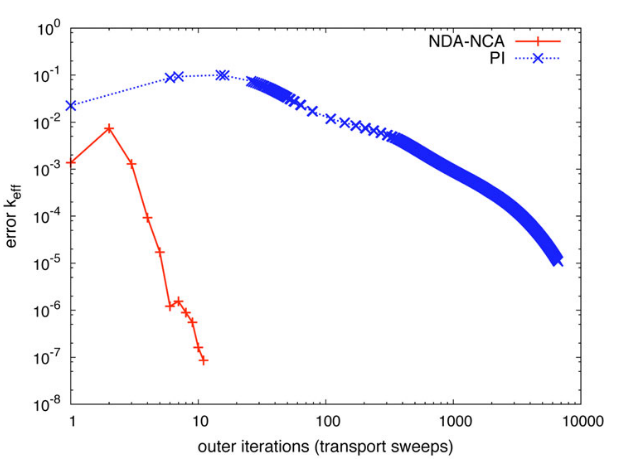
\includegraphics[width=0.5\textwidth]{nda_convergence_park}
    \caption{NDA convergence vs standard power iteration~\cite{Park2012}\label{fig:nda_convergence}}
  \end{figure}
\end{frame}

\begin{frame}
  \frametitle{Analysis challenges}
  \pause
  \begin{block}{Challenge}
    Work definition requires (good) assumptions about algorithm efficiency.
  \end{block}
  \pause
    \begin{equation*}
    \sum_{\ell = 1}^{N'}w'_{(\ell)} <  \sum_{\ell = 1}^Nw_{(\ell)}
  \end{equation*}
  \pause
    \begin{equation*}
    N'w'_{(\text{inv})} <  Nw_{{(\text{inv})}}
  \end{equation*}
  \pause
  Relying on the number of sweeps as a measure of effectiveness relies
  on $w'_{(\text{inv})} \approx  w_{{(\text{inv})}}$.
  \pause
  \begin{block}{}
    This becomes complicated as our acceleration methods become more
    complex, and take on more work.
  \end{block}
\end{frame}

\begin{frame}
  \frametitle{Validating our methods}
  \pause
  \begin{block}{Challenge}
    We want to validate \textit{why} our methods work.
  \end{block}
  \pause
  \begin{itemize}[<+->]
  \item The methods we develop are backed up by math and our
    understanding of the problem.
  \item If a method is successful in accelerating a solve, it's not
    always clear why.
  \item Combinations of methods may make the mathematical analysis difficult or impossible.
  \end{itemize}
  \pause
  \begin{block}{What do we need?}
    Additional, good data that enables us to assess the effectiveness
    of our method.
  \end{block}
\end{frame}

\begin{frame}
  \frametitle{Analysis Challenges}
  A few challenges when analyzing the effectiveness of acceleration
  schemes include:
  \begin{itemize}[<+->]
  \item Work definition requires assumptions about algorithm
    efficiency.
  \item We need good data to show us \textit{why} our methods are working.
  \item Combined or complex schemes may invalidate assumptions.
  \item Implementation and reproducibility can be difficult.
  \end{itemize}
  
  \note{
  \begin{itemize}
  \item Our definition of work is based on assumptions about
    algorithmic efficiency of the entire transport solve.
  \item Combining or using complex acceleration schemes may invalidate
    these assumptions.
  \item Implementing new schemes can be complicated, making it
    difficult to dis-aggregate implementation from theory. 
  \item It can be difficult to reproduce results when accelerated
    codes are not portable.
  \end{itemize}
    }
  
  \end{frame}

% -- When this work assumption breaks down
% - Race car analogy
% -- First past-the-post assessment
% -- Need a standard test track with a standard car that is accessible
% - Motivation for a new tool -- test track
% BART Code Goals (10 min)
\section{Design paradigm}
% - Design goals
\begin{frame}
  \frametitle{Design goals for BART}
  The Bay Area Radiation Transport (BART) is motivated by three major
  design goals. To create a code that,
  \vspace{1em}
  \begin{enumerate}
    \setlength\itemsep{1em}
  \item<2-> relieves some of the burden of implementing a novel acceleration method,
  \item<3-> provides a controlled environment for measuring the
    effectiveness of the novel method, and,
  \item<4-> provides tools for verifying the basis for effectiveness.
  \end{enumerate}  
\end{frame}
% -- Reliving some development burden
\begin{frame}
  \frametitle{Designed for implementation} % 2 minutes
    \begin{block}{Goal 1}Relieving some of the burden of implementing a novel
    acceleration method.
    \end{block}

  \onslide<2->{
  BART is designed to be a code focused on a \textbf{developer}
  end-user.}
  \(
  \<{0.5\textwidth}
  \begin{itemize}    \setlength\itemsep{1em}
  \item<3-> Focus on clarity of structure instead of performance
    (optimization for modification).
  \item<4-> Heavy usage of polymorphism.
  \item<5-> Comprehensive testing coverage.
  \end{itemize}
  \>
  
  \<{0.5\textwidth}
  \only<4>{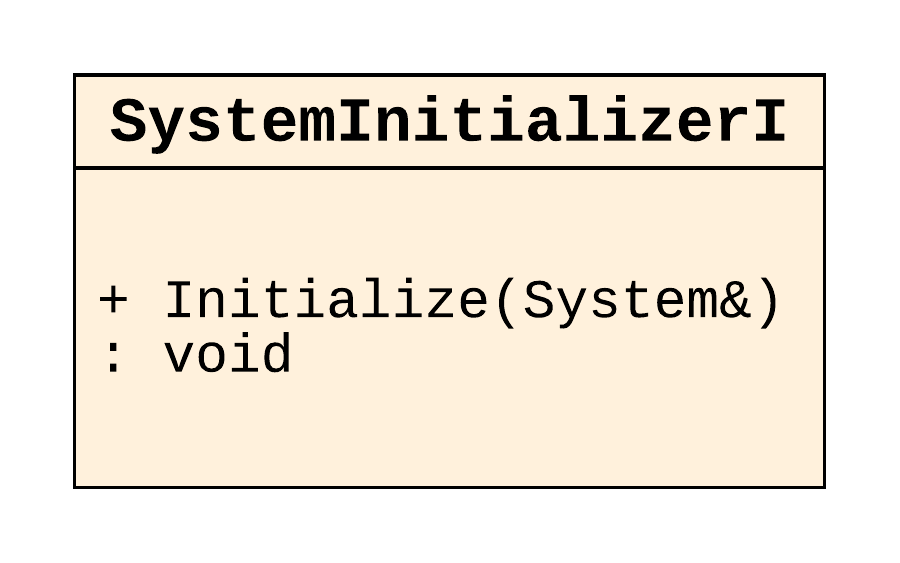
\includegraphics[width=\textwidth]{initializer_interface}}
  \only<5>{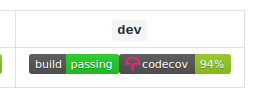
\includegraphics[width=0.75\textwidth]{travis}}
  \>
  \)
\end{frame}
% -- Provide a controlled environment
\begin{frame}
  \frametitle{Controlled testing environment} % 2 minutes
    \begin{block}{Goal 2}Providing a controlled environment for
      measuring the effectiveness of the novel method.
    \end{block}

  \onslide<2->{
    BART is designed to leverage polymorphism to isolate and minimize
    changes required to implement novel methods.}\vspace{1em}
  \onslide<3->{
  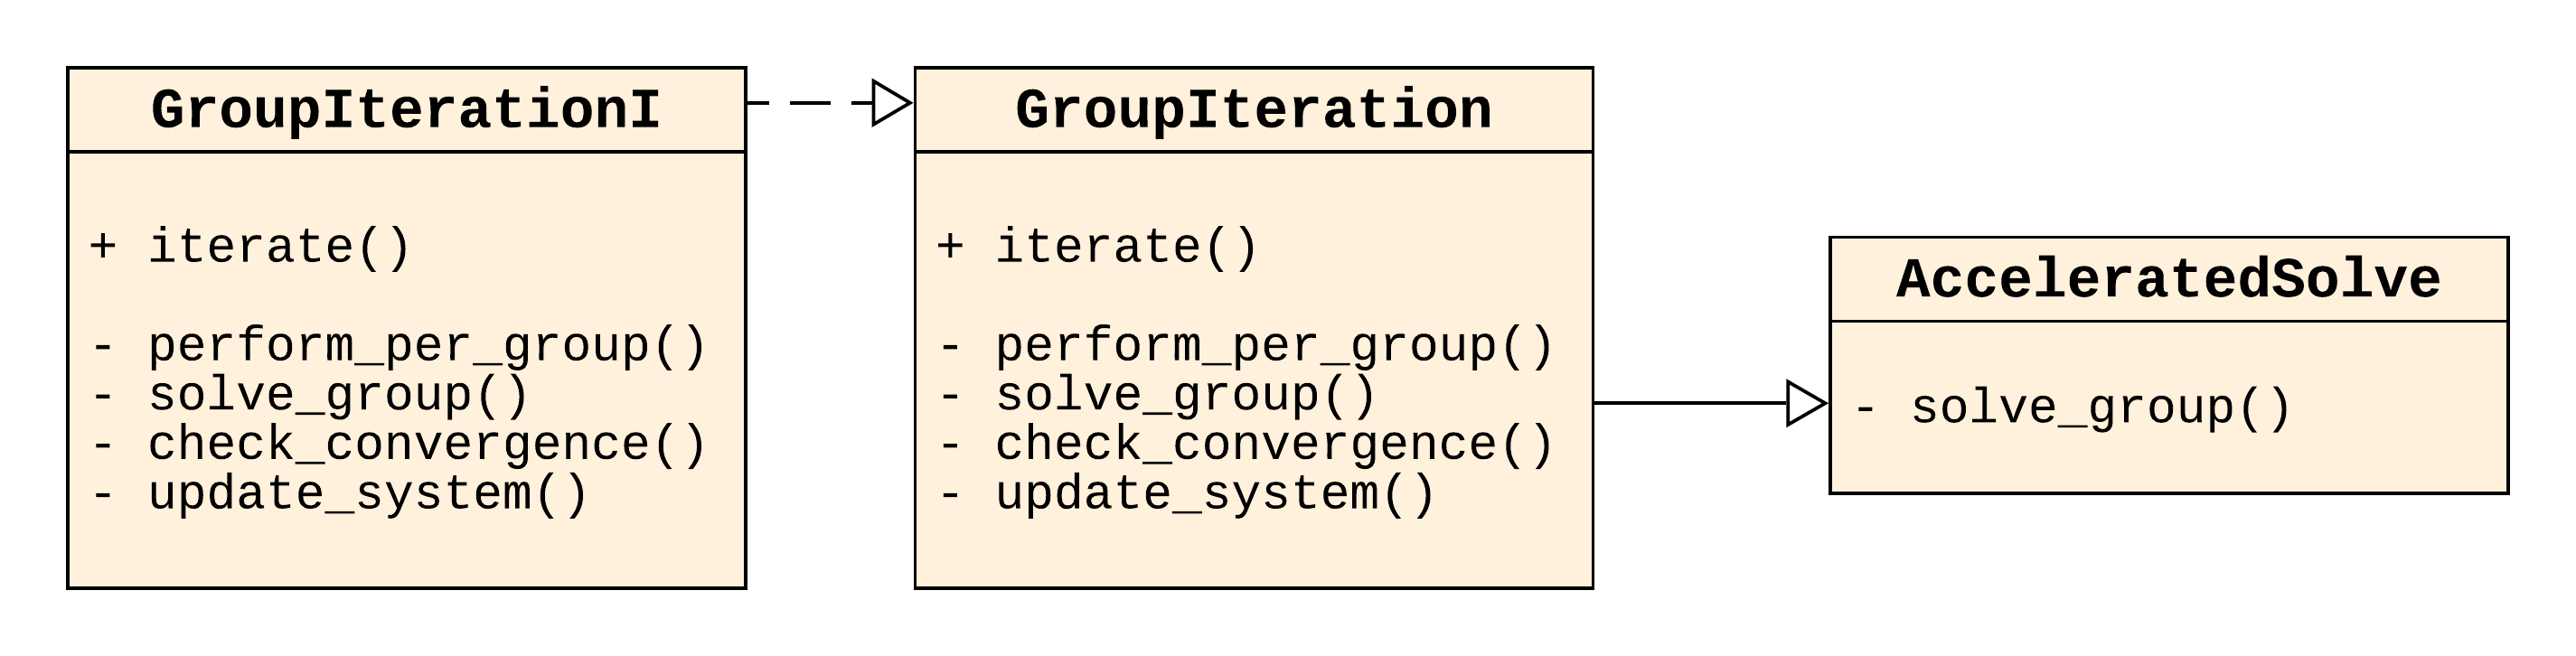
\includegraphics[width=\textwidth]{polymorphism}
  }
\end{frame}
\begin{frame}
  \frametitle{Polymorphism Benefits}
  The use of polymorphism in BART
  \begin{itemize}
  \item<1-> Minimizes code changes needed to implement new methods,
    making it faster and easier.
  \item<2-> Enables a true comparison of the accelerated solve to a
    control solve.
  \item<3-> Makes the modifications \textit{portable}.    
  \item<4-> Enables us to compare the implementation of the method to
    dis-aggregate the computer science from the method itself.
  \end{itemize}
 
\end{frame}
% -- Provide instrumentation
\begin{frame}
  \frametitle{Instrumentation}
  \pause
  \begin{block}{Goal 3}
    Provide tools for verifying the basis for effectiveness.
  \end{block}
  \pause
  BART will include the ability to \textit{instrument} a solve
  to gather enough data to draw useful conclusions about the effectiveness of
  acceleration schemes.
  \pause
\begin{itemize}
  \item Storage of solve parameters (eigenvalues, fluxes).
  \item Storage of hierarchy of iterations.
  \item Calculation and storage of error or residual.
  \item Analysis of Fourier error modes coefficients.
  \end{itemize}
\pause
  \begin{block}{Important}
    Adding new instrumentation must be easy!
  \end{block}
\end{frame}
% State of the code (2 min)
\begin{frame}
  \frametitle{Goals Reprise}
  To create a code that, 
  \vspace{1em}
  \begin{enumerate}
    \setlength\itemsep{1em}
  \item relieves some of the burden of implementing a novel acceleration method,
  \item provides a controlled environment for measuring the
    effectiveness of the novel method, and,
  \item provides tools for verifying the basis for effectiveness.
  \end{enumerate}

  \begin{block}
    Getting goal three right relies on doing one and two really well.
  \end{block}
\end{frame}
\section{Status and future work}
% - Finite element (1 min)
\begin{frame}
  \frametitle{The BART Code}
  \begin{itemize}[<+->]
  \item Deterministic, finite-element-based transport code.
  \item Coded in \Cpp{}, using the \Cpp[17] standard. A python script can
    automate creation of input files.
  \item Uses the \texttt{deal.II} finite-element library~\cite{dealII90}.
  \item Parallel processor (MPI) calculations are supported using
    PETSc~\cite{petsc-web-page, petsc-user-ref, petsc-efficient}.
  \item Uses the GoogleTest/GoogleMock framework for testing~\cite{googletest}, with
    \texttt{travis.ci} continuous integration.
  \item Uses the Google Protocol Buffers file format for cross-sections.
  \end{itemize}
\end{frame}

\begin{frame}
  \frametitle{Current support and future work}
  \begin{itemize}[<+->]    
  \item Supports 1-, 2-, and 3-D solves.
  \item Two 2nd-order formulations of the transport equation
    implemented: diffusion and self-adjoint angular flux equation.
  \item Acceleration methods in development: nonlinear diffusion
    acceleration (NDA).
  \item Future methods: transport two-grid acceleration (TTG), and a
    combination of NDA and TTG.
  \item Instrumentation in development: \textit{in-situ} stepwise Fourier Analysis.
  \end{itemize}
\end{frame}

\begin{frame}
  \frametitle{Conclusion}
  \pause
  \begin{itemize}[<+->]
  \item Implementing and analyzing acceleration methods has practical
    challenges.
  \item We are developing a new code aimed at helping developers of
    new methods.
  \item We hope that the code will ease the burden of coding up new
    methods, and help provide good, useful data for understanding if
    and why the methods are worthwhile to implement in production
    level codes.
  \end{itemize}
\end{frame}

\begin{frame}[noframenumbering, plain]
  \centering\Large{Thank you}
\end{frame}

% Future work (1 min)
% - More acceleration methods
% - Combinations of acceleration methods

\frame[noframenumbering, plain]{\frametitle{References}
\tiny{\bibliographystyle{plain}}
\bibliography{bib/bib}
}

\appendix

\section{Backup Slides}

\frame[c]{\frametitle{Backup Slide}
  Backup
  }

\end{document}

%%% Local Variables:
%%% mode: latex
%%% TeX-master: t
%%% End:
